\chapter{Background Estimation}
\label{chapter:background_estimation}

% CR and VR N-1 figure source: hepdata or bonly_20260921.
\providecommand{\CHEightCRFigureVersion}{hepdata}

The background estimation uses both simulated samples and data. The simulated samples are used to predict the background yields in the SRs, while data are used to correct mismodelling of the backgrounds.
Since the fake-$\hadtau$ background is small and the signal topology is relatively easy to identify, a simple cut-and-count method is used for background estimation, with dedicated normalisation factors (NFs) for the dominant backgrounds.
Therefore, dedicated control regions (CRs) and validation regions (VRs) are defined to estimate the NFs and validate the background predictions, respectively.
This chapter presents the background estimation strategy, the CR and VR definitions, and the validation of the background predictions after the background-only fit\footnote{The background-only fit is performed by fitting background in the CRs with the background-only hypothesis.}.

\section{Background estimation strategy}
\label{sec:ch8_strategy}

The estimation strategy for each background is summarised below:
\begin{itemize}
    \item $\wjets$ is estimated using NFs constrained by data in $\CRW$, where one light leptonic (electron or muon) and no $\hadtau$ or $b$-jets are required.
    The $0b\to1b$ extrapolation is tested in $\VRW$, where one light lepton, no $\hadtau$ and one $b$-jet are required.

    \item The top-quark background is estimated using NFs constrained by data in $\CRTop$, where one $\hadtau$, one light lepton and at least one $b$-jet are required.
    The prediction is tested in $\VRTop$, where one $\hadtau$, no light leptons and two $b$-jets are required.

    \item $\znunu$ with a jet misidentified as a $\hadtau$ is estimated directly from simulation.
    A conservative uncertainty is assigned based on the study of $\zll$ events with a fake-$\hadtau$ in Appendix~\ref{app:ch8_fake_tau}.

    \item $\ztautau$ and diboson production are estimated directly from simulation without dedicated CRs.
    Their predicted yields are allowed to vary within conservative uncertainties in the fit.

    \item The multijet background is negligible after the full SR selections, including the suppression described in Section~\ref{subsec:ch7_multijet}, as checked in Appendix~\ref{App:QCD_bkg_study}.
\end{itemize}

Four CRs are therefore defined in this analysis: $\CRW$-$\Res$ and $\CRW$-$\NonRes$ for $\wjets$, and $\CRTop$-$\Res$ and $\CRTop$-$\NonRes$ for the top-quark background, corresponding to the normalisation factors $\lambda_W^{\Res}$, $\lambda_W^{\NonRes}$, $\lambda_t^{\Res}$ and $\lambda_t^{\NonRes}$, respectively. They are defined as follows:
\begin{equation}
    \lambda_{bg} = \frac{N_{bg}^{\mathrm{CR,data}}}{N_{bg}^{\mathrm{CR,MC}}}.
    \label{eq:ch8_lambda}
\end{equation}
where $N_{bg}^{\mathrm{CR,data}}$ and $N_{bg}^{\mathrm{CR,MC}}$ are the observed and the predicted background event yields in the CR, respectively.
The independent NFs allow different normalisation in the resonant and non-resonant regions, which probe different $\pT$ ranges.
The VRs do not participate in the fit.
Residual mismodelling of the small contribution from the top-quark background in $\CRW$ can be partly absorbed by a shift in $\lambda_W$, and vice versa.
The SR, CR and VR definitions are summarised in Figure~\ref{fig:ch8_region_definition}.
\begin{figure}[htpb]
    \centering
    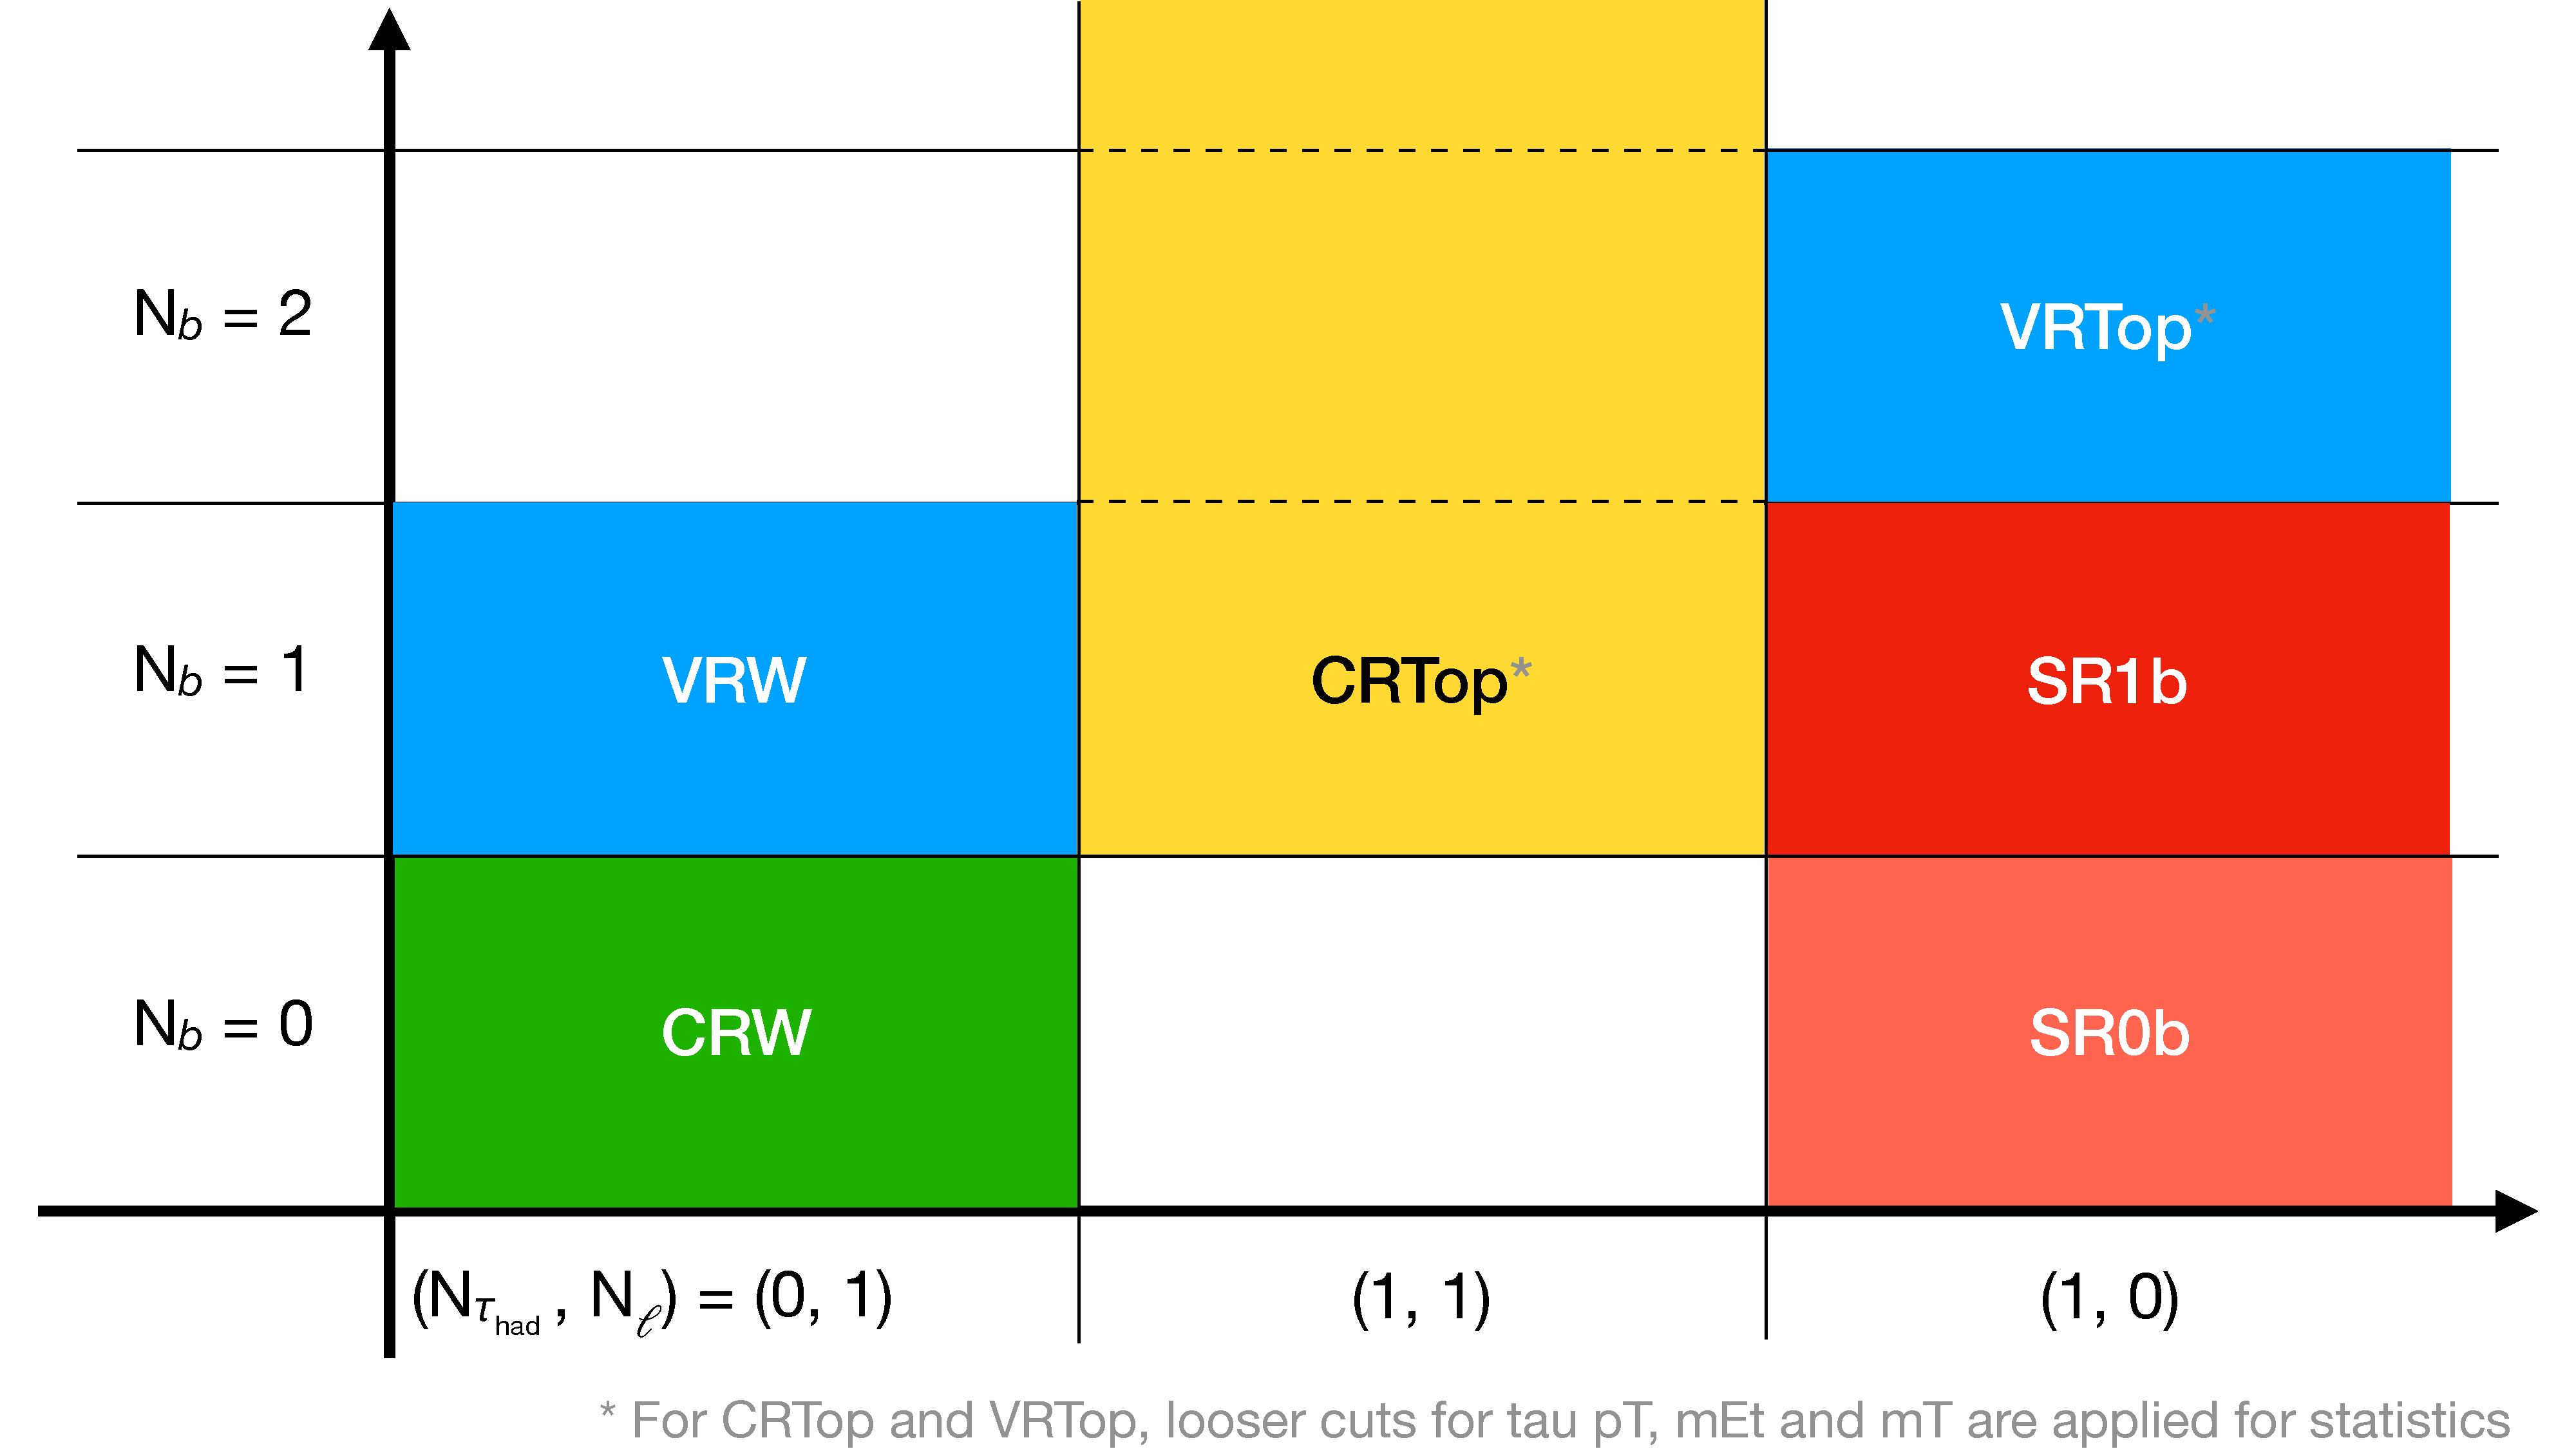
\includegraphics[width=0.95\linewidth]{Figs/CH8/RegionDefinitions.pdf}
    \caption[SR, CR and VR definitions]{SR, CR and VR definitions in terms of the $\hadtau$, light-lepton and $b$-jet multiplicities. Separate resonant and non-resonant regions are defined for each.}
    \label{fig:ch8_region_definition}
\end{figure}

\section[W+jets]{$\wjets$}
\label{sec:ch8_wjets}

The $\CRW$ regions are defined by replacing the $\hadtau$ lepton in the SR selection with an light lepton, targeting the $W\to\ell\nu$ process.
The $b$-jet veto suppresses the top-quark background and increases the $\wjets$ event purity.
Single-lepton triggers are used, as listed in Table~\ref{tab:run2_trigger_chains}.
This avoids differences in the $\met$ trigger response between the electron and muon channels, since the muon momentum is not included in the trigger-level $\met$ calculation.
$\mT^\ell$ and $\DphiLepMet$ are calculated using the light lepton as a proxy for the $\hadtau$ lepton, and the leading jet is used as a proxy for the $b$-jet. The other selections are the same as the SRs.

The definitions of the $\CRW$ and $\VRW$ regions are summarised in Table~\ref{tab:ch8_wcr_vrw}.
After the background-only fit, the $\wjets$ purity is approximately $95\%$ in $\CRW$-$\NonRes$ and $82\%$ in $\CRW$-$\Res$. Diboson events are expected to contribute approximately $14\%$ in $\CRW$-$\Res$.
The additional neutrino in a hadronic $\tau$ decay introduces kinematic differences in the $1\ell\to1\hadtau$ extrapolation. The prediction is further tested in the lower-mass $1\hadtau0\ell1b$ regions described in Section~\ref{subsec:low_mass_vr}, which check the extrapolation to events with both a $\hadtau$ and a $b$-jet.

Signal contamination is checked with samples including both hadronic and leptonic $\tau$ decays at parameter points $(\MU,\gU,\beta_L^{23})=(1.5~\TeV,1.5,0.2)$ and $(2.5~\TeV,1.5,1.0)$ for the resonant and non-resonant CRs, respectively. The contamination is found to be below $1\%$ in both regions.

\begin{table}[htbp]
    \centering
    \small
    \caption[Event selections for $\CRW$ and $\VRW$]{Event selections for $\CRW$ and $\VRW$. Differences from SRs are shown in bold. The selected jet is the leading jet in $\CRW$ and the $b$-jet in $\VRW$.}
    \label{tab:ch8_wcr_vrw}
    \begin{tabular}{lcc}
        \toprule
        Requirement & \multicolumn{2}{c}{$\CRW$ and $\VRW$ selections} \\
        \midrule
        Trigger & \multicolumn{2}{c}{\textbf{Lowest-unprescaled single-lepton trigger}} \\
        $\hadtau$ multiplicity & \multicolumn{2}{c}{$\bm{N_{\hadtau}=0}$} \\
        $b$-jet multiplicity & \multicolumn{2}{c}{$\bm{N_b=0}$ in $\CRW$, $N_b=1$ in $\VRW$} \\
        Light-lepton multiplicity & \multicolumn{2}{c}{$\bm{N_\ell=1}$} \\
        Multijet suppression & \multicolumn{2}{c}{$\minDphiJetMet>0.4\quad\text{or}\quad\metOverMinDphiJetPt>6$} \\
        \midrule
         & Resonant & Non-resonant \\
        \midrule
        $\pT^\mathrm{jet}$ [$\GeV$] & $>250$ & $[50, 250]$ \\
        $\DphiLepMet$ & N/A & $>1.2$ \\
        $\met$ [$\GeV$] & $>200$ & $>400$ \\
        $\pT^\ell$ [$\GeV$] & $>200$ & $>200$ \\
        $\mT^\ell$ [$\GeV$] & $>200$ & $>600$ \\
        $m_{j\ell}$ or $m_{b\ell}$ [$\GeV$] & $>800$ & N/A \\
        $N_j$ & $\leq4$ & $\leq2$ \\
        \bottomrule
    \end{tabular}
\end{table}

The $\CRW$ $N-1$ distributions after the background-only fit are shown separately for the electron and muon channels in Figures~\ref{fig:ch8_wcr_res_e}--\ref{fig:ch8_wcr_nonres_mu}.
There are 243 electron and 219 muon events in $\CRW$-$\Res$, and 474 electron and 398 muon events in $\CRW$-$\NonRes$.
No clear slope is observed in the data/bkg. ratios, except in the jet-$\pT$ distribution in Fig.~\ref{fig:ch8_wcr_nonres_mu}(\subref{fig:ch8_wcr_nonres_mu_jetpt}).
The average effect of this jet-$\pT$ dependence in each region is expected to be absorbed by the independent $\wjets$ normalisation factors.

The difference between the data/bkg. ratios of the electron and muon channels is consistent with statistical fluctuations, as shown in Appendix~\ref{app:ch8_emu}.
The two channels are therefore combined.

\input{Chapters/background_estimation/figures_wcr_\CHEightCRFigureVersion}
\clearpage

\section[Top-quark background]{Top-quark background}
\label{sec:ch8_top}

The $\CRTop$ regions are defined by replacing the light-lepton veto in the SR selection with exactly one light lepton to correct the modelling through $\ttbar\to b\tau\nu\,\bar b\ell\nu$ and $Wt\to b\tau\nu\,\ell\nu$ processes.
Since few top-quark background events pass the high-$\mT$ requirement, single-lepton triggers are used to allow a lower $\met$ threshold than in the SRs and increase the CR yields.

To further increase the CR yields, at least one $b$-jet is required instead of exactly one. The shape comparison in Appendix~\ref{app:ch8_topcr_1b2b} supports combining the one- and two-$b$-jet samples. The $\pT^{\hadtau}$ and $\mT$ thresholds are also lowered, and no $m_{b\hadtau}$ requirement is applied.
The leading $b$-jet is used to calculate the $b$-related variables in case multiple $b$-jets are selected.
The other selections are the same as the ones in SRs.

The $\CRTop$ definition is summarised in Table~\ref{tab:ch8_top_regions}.
The top-quark background purity is approximately $90\%$ in both $\CRTop$ regions.
Signal contamination is negligible because the additional light lepton is not expected in the signal topology.

\begin{table}[htbp]
    \centering
    \small
    \caption[Event selections for $\CRTop$]{Event selections for $\CRTop$. Differences from SRs are shown in bold.}
    \label{tab:ch8_top_regions}
    \begin{tabular}{lcc}
        \toprule
        Requirement & \multicolumn{2}{c}{\textbf{$\CRTop$ selections}} \\
        \midrule
        Trigger & \multicolumn{2}{c}{\textbf{Lowest-unprescaled single-lepton trigger}} \\
        $\hadtau$ multiplicity & \multicolumn{2}{c}{$N_{\hadtau}=1$} \\
        $b$-jet multiplicity & \multicolumn{2}{c}{$\bm{N_b\geq1}$} \\
        Light-lepton multiplicity & \multicolumn{2}{c}{$\bm{N_\ell=1}$} \\
        Multijet suppression & \multicolumn{2}{c}{$\minDphiJetMet>0.4\quad\text{or}\quad\metOverMinDphiJetPt>6$} \\
        \midrule
        $\pT^\ell$ [$\GeV$] & \multicolumn{2}{c}{$>28$} \\
        $\met$ [$\GeV$] & \multicolumn{2}{c}{$\bm{>100}$} \\
        $\pT^{\hadtau}$ [$\GeV$] & \multicolumn{2}{c}{$\bm{>100}$} \\
        $\mT$ [$\GeV$] & \multicolumn{2}{c}{$\bm{>100}$} \\
        $m_{b\hadtau}$ [$\GeV$] & \multicolumn{2}{c}{\textbf{N/A}} \\
        \midrule
         & Resonant & Non-resonant \\
        \midrule
        $\pT^b$ [$\GeV$] & $>250$ & $[50, 250]$ \\
        $\DphiTauMet$ & N/A & $>1.2$ \\
        $N_j$ & $\leq4$ & $\leq2$ \\
        \bottomrule
    \end{tabular}
\end{table}

The $\VRTop$ regions are used to test the extrapolation from $\CRTop$ to final states without a light lepton, as in the SRs.
Exactly two $b$-jets are required to enrich the top-quark background and avoid overlap with $\bTagSR$.
The leading $b$-jet is used to calculate the $b$-jet kinematic variables.
The $\pT^{\hadtau}$ and $m_{b\hadtau}$ thresholds are lowered to gain more statistics.
The selections are summarised in Table~\ref{tab:ch8_vrtop_regions}.

\begin{table}[htbp]
    \centering
    \small
    \caption[Event selections for $\VRTop$]{Event selections for $\VRTop$. Differences from SRs are shown in bold.}
    \label{tab:ch8_vrtop_regions}
    \begin{tabular}{lcc}
        \toprule
        Requirement & \multicolumn{2}{c}{\textbf{$\VRTop$ selections}} \\
        \midrule
        Trigger & \multicolumn{2}{c}{Lowest-unprescaled $\met$ trigger} \\
        $\hadtau$ multiplicity & \multicolumn{2}{c}{$N_{\hadtau}=1$} \\
        $b$-jet multiplicity & \multicolumn{2}{c}{$\bm{N_b=2}$} \\
        Light-lepton multiplicity & \multicolumn{2}{c}{$N_\ell=0$} \\
        Multijet suppression & \multicolumn{2}{c}{$\minDphiJetMet>0.4\quad\text{or}\quad\metOverMinDphiJetPt>6$} \\
        \midrule
         & Resonant & Non-resonant \\
        \midrule
        $\pT^b$ [$\GeV$] & $>250$ & $[50, 250]$ \\
        $\DphiTauMet$ & N/A & $>1.2$ \\
        $\met$ [$\GeV$] & $>200$ & $\bm{>200}$ \\
        $\pT^{\hadtau}$ [$\GeV$] & $\bm{>100}$ & $\bm{>100}$ \\
        $\mT$ [$\GeV$] & $\bm{>100}$ & $\bm{>200}$ \\
        $m_{b\hadtau}$ [$\GeV$] & $\bm{>400}$ & N/A \\
        $N_j$ & $\leq4$ & $\leq2$ \\
        \bottomrule
    \end{tabular}
\end{table}

The $\CRTop$ $N-1$ distributions after the background-only fit are shown separately for the electron and muon channels in Figures~\ref{fig:ch8_topcr_res_e}--\ref{fig:ch8_topcr_nonres_mu}.
There are 30 electron and 33 muon events in $\CRTop$-$\Res$, and 240 electron and 228 muon events in $\CRTop$-$\NonRes$.
Similar behaviour is observed in the two lepton channels with no clear slope in the data/bkg. ratios.
The electron and muon channels are therefore combined.


\input{Chapters/background_estimation/figures_topcr_\CHEightCRFigureVersion}
\clearpage

\section{Background-only fit and validation}
\label{sec:ch8_validation}

The background-only fit is performed on the CRs to obtain the background normalisation factors.
Both statistical and systematic uncertainties are included in the fit. The fit model and systematic uncertainties are described in detail in Section~\ref{sec:ch10_statistical_model} and Chapter~\ref{chapter:systematics_uncertainties}, respectively.
The four fitted NFs are summarised in Table~\ref{tab:ch8_normalisation}.
The difference between $\lambda_W^{\Res}$ and $\lambda_W^{\NonRes}$ is consistent with the expectation discussed in Section~\ref{sec:ch8_wjets}.
The background predictions are tested in the VRs defined in Figure~\ref{fig:ch8_region_definition}.

\begin{table}[htbp]
    \centering
    \caption[Background normalisation factors from the CR fit]{Background normalisation factors from the background-only fit on CRs. Both statistical and systematic uncertainties are included in the fit.}
    \label{tab:ch8_normalisation}
    \begin{tabular}{lcc}
        \toprule
        Background & Resonant & Non-resonant \\
        \midrule
        $\lambda_W$ & $1.21\pm0.11$ & $0.89\pm0.08$ \\
        $\lambda_t$ & $0.76\pm0.16$ & $0.81\pm0.16$ \\
        \bottomrule
    \end{tabular}
\end{table}

\subsection[VRW]{$\VRW$}
\label{subsec:ch8_vrw}

As in SRs, the background in $\VRW$ is dominated by $\wjets$, which contributes approximately $66.5\%$ ($68.4\%$) in the resonant (non-resonant) region after the background-only fit.
Top-quark and diboson production contribute approximately $22.7\%$ ($28.6\%$) and $9.6\%$ ($2.9\%$), respectively.

Signal contamination is checked using samples introduced in Section~\ref{sec:ch8_wjets}.
% Direct signal production with an electron or muon is suppressed by the small couplings to these leptons, while hadronic $\tau$ decays contribute little to the selected sample.
The contribution from leptonic $\tau$ decays is $(1.3\pm0.1)\%$ in $\VRW$-$\Res$ and $(0.7\pm0.1)\%$ in $\VRW$-$\NonRes$, while the contribution from hadronic $\tau$ decays is negligible.

After the background-only fit, the $\VRW$-$\Res$ yield agrees with the prediction within about $1\sigma$, while a deviation of about $2\sigma$ is observed in the $\VRW$-$\NonRes$ region.
The post-fit $N-1$ distributions are shown in Figures~\ref{fig:ch8_vrw_res} and~\ref{fig:ch8_vrw_nonres}.
Checks with finer $\met$ bins and different $\met$ thresholds show that the excess is localised in $425<\met<450~\GeV$. And the neighbouring $\met$ regions show better agreement between data and prediction.
No indication of a local detector problem is found in the $(\eta,\phi)$ distributions of the leptons and $b$-jets.
Good agreement is also found in the additional low-mass VRs.
These results identify no specific modelling problem and are consistent with the excess being a statistical fluctuation. More details are presented in Appendix~\ref{app:ch8_vrw_excess}.

\input{Chapters/background_estimation/figures_vrw_\CHEightCRFigureVersion}
\subsection[VRTop]{$\VRTop$}
\label{subsec:ch8_vrtop}

The background in $\VRTop$ is dominated by top-quark production with fractions of approximately $67\%$ and $86\%$ in the resonant and non-resonant regions, respectively.
Specifically, single-top and $\ttbar$ production contribute approximately $35\%$ and $32\%$ of the total background in the resonant region, respectively, while $\ttbar$ dominates the non-resonant region with a contribution of approximately $80\%$.
Signal contamination is checked using the same samples and benchmarks as in $\VRW$, which is $(1.2\pm0.1)\%$ in $\VRTop$-$\Res$ and $(0.6\pm0.03)\%$ in $\VRTop$-$\NonRes$.

After the background-only fit, the expected yields are $13.0\pm3.9$ and $30.1\pm8.1$ in $\VRTop$-$\Res$ and $\VRTop$-$\NonRes$, compared with 19 and 30 observed events, respectively. The observed yields agree with the predictions within about $1\sigma$ in both regions.
The post-fit $N-1$ distributions are shown in Figures~\ref{fig:ch8_vrtop_res} and~\ref{fig:ch8_vrtop_nonres}.
The agreement supports the extrapolation from $\CRTop$ to final states without a light lepton.

\input{Chapters/background_estimation/figures_vrtop_\CHEightCRFigureVersion}
\clearpage
